\documentclass{article}
% Change "article" to "report" to get rid of page number on title page
\usepackage{amsmath,amsfonts,amsthm,amssymb}
\usepackage{setspace}
\usepackage{Tabbing}
\usepackage{fancyhdr}
\usepackage{lastpage}
\usepackage{extramarks}
\usepackage{chngpage}
\usepackage{soul,color}
\usepackage{graphicx,float,wrapfig}
\usepackage{multirow}
\usepackage{enumerate}
% In case you need to adjust margins:
\topmargin=-0.45in      %
\evensidemargin=0in     %
\oddsidemargin=0in      %
\textwidth=6.5in        %
\textheight=9.0in       %
\headsep=0.25in         %

% Homework Specific Information
\newcommand{\hmwkTitle}{Annealed ME}
\newcommand{\hmwkClass}{}
\newcommand{\hmwkAuthorName}{Donglai\ Wei}


% Setup the header and footer
\pagestyle{fancy}                                                       %
\lhead{\hmwkAuthorName}                                                 %
\rhead{\firstxmark}                                                     %
\lfoot{\lastxmark}                                                      %
\cfoot{}                                                                %
\rfoot{Page\ \thepage\ of\ \pageref{LastPage}}                          %
\renewcommand\headrulewidth{0.4pt}                                      %
\renewcommand\footrulewidth{0.4pt}                                      %

% This is used to trace down (pin point) problems
% in latexing a document:
%\tracingall

%%%%%%%%%%%%%%%%%%%%%%%%%%%%%%%%%%%%%%%%%%%%%%%%%%%%%%%%\begin{enumerate}

% Some tools
\newcommand{\enterProblemHeader}[1]{\nobreak\extramarks{#1}{#1 continued on next page\ldots}\nobreak%
                                    \nobreak\extramarks{#1 (continued)}{#1 continued on next page\ldots}\nobreak}%
\newcommand{\exitProblemHeader}[1]{\nobreak\extramarks{#1 (continued)}{#1 continued on next page\ldots}\nobreak%
                                   \nobreak\extramarks{#1}{}\nobreak}%

\newlength{\labelLength}
\newcommand{\labelAnswer}[2]
  {\settowidth{\labelLength}{#1}%
   \addtolength{\labelLength}{0.25in}%
   \changetext{}{-\labelLength}{}{}{}%
   \noindent\fbox{\begin{minipage}[c]{\columnwidth}#2\end{minipage}}%
   \marginpar{\fbox{#1}}%

   % We put the blank space above in order to make sure this
   % \marginpar gets correctly placed.
   \changetext{}{+\labelLength}{}{}{}}%

\setcounter{secnumdepth}{0}
\newcommand{\homeworkProblemName}{}%
\newcounter{homeworkProblemCounter}%
\newenvironment{homeworkProblem}[1][Problem \arabic{homeworkProblemCounter}]%
  {\stepcounter{homeworkProblemCounter}%
   \renewcommand{\homeworkProblemName}{#1}%
   \section{\homeworkProblemName}%
   \enterProblemHeader{\homeworkProblemName}}%
  {\exitProblemHeader{\homeworkProblemName}}%

\newcommand{\problemAnswer}[1]
  {\noindent\fbox{\begin{minipage}[c]{\columnwidth}#1\end{minipage}}}%

\newcommand{\problemLAnswer}[1]
  {\labelAnswer{\homeworkProblemName}{#1}}

\newcommand{\homeworkSectionName}{}%
\newlength{\homeworkSectionLabelLength}{}%
\newenvironment{homeworkSection}[1]%
  {% We put this space here to make sure we're not connected to the above.
   % Otherwise the changetext can do funny things to the other margin

   \renewcommand{\homeworkSectionName}{#1}%
   \settowidth{\homeworkSectionLabelLength}{\homeworkSectionName}%
   \addtolength{\homeworkSectionLabelLength}{0.25in}%
   \changetext{}{-\homeworkSectionLabelLength}{}{}{}%
   \subsection{\homeworkSectionName}%
   \enterProblemHeader{\homeworkProblemName\ [\homeworkSectionName]}}%
  {\enterProblemHeader{\homeworkProblemName}%

   % We put the blank space above in order to make sure this margin
   % change doesn't happen too soon (else \sectionAnswer's can
   % get ugly about their \marginpar placement.
   \changetext{}{+\homeworkSectionLabelLength}{}{}{}}%

\newcommand{\sectionAnswer}[1]
  {% We put this space here to make sure we're disconnected from the previous
   % passage

   \noindent\fbox{\begin{minipage}[c]{\columnwidth}#1\end{minipage}}%
   \enterProblemHeader{\homeworkProblemName}\exitProblemHeader{\homeworkProblemName}%
   \marginpar{\fbox{\homeworkSectionName}}%

   % We put the blank space above in order to make sure this
   % \marginpar gets correctly placed.
   }%

%%%%%%%%%%%%%%%%%%%%%%%%%%%%%%%%%%%%%%%%%%%%%%%%%%%%%%%%%%%%%



%%%%%%%%%%%%%%%%%%%%%%%%%%%%%%%%%%%%%%%%%%%%%%%%%%%%%%%%%%%%%
% Make title
\title{\vspace{0.3in}\textmd{\textbf{\hmwkTitle}}}
\date{2010.6.24}
\author{\textbf{\hmwkAuthorName}}
%%%%%%%%%%%%%%%%%%%%%%%%%%%%%%%%%%%%%%%%%%%%%%%%%%%%%%%%%%%%%

\begin{document}
\begin{spacing}{1.1}
\maketitle
\section{0) Notations }
Hierarchical Dirichlet Process Model with Dirichlet-Multinomial:
\subsection{i)Formula}
$n_{jtk}$number of customers in table t, restaurant j, with dish k \\
$m_{jk}$number of tables in restaurant j, with dish k \\ 
$n_{..k}$number of customers in dish k \\
$n_{..k}^{w}$number of occurence of word w in dish k \\
$n_{j..}$number of customers in in Restaurant j \\
$n_{jt.}$number of customers in table t in Restaurant j \\
$m_{..}$number of tables in total \\
$m_{.k}$number of tables in dish k \\ 
J Restaurants,K dishes\\ \\
{\bf a) Goal}:(Marginalize $\theta$ and Search over z:)\\
 Maximize log Probability $L=log p(x,z|\lambda)$\\ =\\
(t-term)$ \underline{log \frac{\Gamma(\gamma)}{\Gamma(m_{..}+\gamma)}+\sum_{j=1}^{J} \{log \frac{\Gamma(\alpha)}{\Gamma(n_{j..}+\alpha)}+\sum_{t=1}^{m_{j.}}[log(\Gamma(n_{jt.}))+log \alpha
]\}}$\\ \\
+(k-term)$ \sum_{k=1}^{K} [log(\frac{\Pi_{w=1}^{W}\Gamma(\lambda_{0}+n_{..k}^{w})}{\Gamma(n_{..k}+W\lambda_{0})})+log(\frac{\Gamma(W\lambda_{0})}{\Gamma(\lambda_{0})^{W}})
+\underline{log(\Gamma(m_{.k}))+log \gamma]}$\\ \\ \emph{{\small (underlined part come from Hierarchical Dirichlet Process)}}\\ \\ \\
{\bf b) Annealing}: Maximize the annealed log Probability:\\ \\
L'(Temperature)=Temperature*(t-term)+(k-term)

\newpage

\section{1) ME algorithm: }
\subsection{i) Unified Backbone}
\begin{enumerate}[(1)]
\item Annealing:(n:number of iterations; p:annealing power)
\begin{enumerate}[(i)]
\item For iter=1:n
\item Temperature=$(\frac{iter}{n})^p$
\item Decompose Restaurants(Temperature)
\item {\color{red}{Merge Dish(Temperature)}}
\item End
\end{enumerate}
\item Running for Convergence:
\begin{enumerate}[(i)]
\item While L doesn't increase any more
\item Decompose Restaurants(1)
\item {\color{red}{Merge Dish(1)}}
\item End
\end{enumerate}
\end{enumerate}

\subsection{ii) Decompose Restaurants(Temperature)}
For j=Randperm(J)
\begin{enumerate}[(A)]
\item Rough reconfiguration for Restaurant j:
\begin{enumerate}[(i)]
\item Make Restaurant j into one table $t_{0}$ where customers following uniform distribution:\\
\small{\emph{($\%$Thus the Probability P($t_{ji}=t_{0}$)=$\frac{1}{W}$)}}
\item Possible Dish=$\{Nonempty \ dishes\}$
\item While Possible Dish is not empty:
\begin{enumerate}[(a)]
\item For each dish k$\in$Possible Dish, propose to form a new table $t_{k}$ out of $t_{0}$ with dish k and calculate {\color{red}{the change for these two dishes}} $\Delta k$:\\
\small{\emph{($\%$For each customer i in $t_{0}$, sample $t_{ji}\in\{t_{0},t_{k}\}\sim\{\frac{1}{W},\frac{n_{..k}^{w}+\phi}{n_{..k}+W\phi}\}$)}}\\
\small{\emph{($\%$Propose to form table $t_{k}$ with customers whose $t_{ji}=t_{k}$)}}
Sample a proposal $t_{k*}$ according to the weight and make the new table:\\
\small{\emph{($\%$Sample a proposal $\{t_{k_{1}},...,t_{k_{K}}\}\sim e^{r_{proposal}\{\Delta k_{1},...\Delta k_{K}\}}$)}}\\
\small{\emph{($\%r_{proposal}>0$, the more decrease of $\Delta k$, the less propable to form table $t_{k}$)}}
\item Possible Dish=Possible Dish$\setminus k_{*}$
\end{enumerate}
\item If there are still customers left in $t_{0}$,make it a new table with a new dish
\end{enumerate}

\item Refined reconfiguration for Restaurant j:TKM(j,{\bf Temperature}):\\
\small{\emph{($\%$Divide the change of L between present Restaurant j config and its previous config into t-term,k-term change: $\Delta L$=$\Delta K$+$\Delta T$)}}
\item Decision:\\
{\color{red}{If($\Delta K+{\bf Temperature}*\Delta T<$0):}}\\
Accept the new configuration\\ 
else:\\
Restore Previous Config\\
\end{enumerate}
End
\subsection{iii) Merge Dish(Temperature)}
 Dish List=$\{Nonempty \ dishes\}$\\ \\
 While Dish List is not empty:\\
 1) Randomly pick a dish k$\in$ Dish List\\
 2) Dish List=Dish List$\setminus$k\\
 3) Merge dish k to the dish$\in$ Dish List which increase {\bf L'(Temperature)} mostly\\(if cannot increase {\bf L'(Temperature)}, then leave it alone)\\
 End\\


\subsection{iv) TKM(Restaurant index,Temperature)}
While {\bf L'(Temperature)} doesn't increase any more:
\begin{enumerate}[(A)]
\item Local Search Table:\\ \\
For $t_{1}$=Randperm($m_{j.}$):\\
For $t_{2}$=Randperm($m_{j.}\setminus t_{1}$):\\ \\
While local move can be made:\\
Greedily move one customer at a time from $t_{1}$ to $t_{2}$ if the move increases L \\
End\\ \\
End\\End
\item Local Search Dish:\\ \\
For $t_{1}$=Randperm($m_{j.}$):\\
Assign $t_{1}$ to the dish which increase L most(allow it to have new dish)\\
End
\item Merge table:\\ \\
 For $t_{1}$=Randperm($m_{j.}$):\\
 Merge table $t_{1}$ to the table in j which increase {\bf L'(Temperature)} most\\(if cannot increase {\bf L'(Temperature)},then leave it alone)\\
 End\\ \\
\end{enumerate}  
End
\newpage
\section{2) Anealing}
Things to play with:
\begin{enumerate}
 \item Parameters to tune:
\begin{enumerate}
\item Annealing Scheme:n:number of iterations; p:annealing power
\item $r_{proposal}$:constant or annealed? (we may want it peaky in the beginning and allow more variability later on)
\end{enumerate}
\item Functions to Anneal:("Merge table" is annealed,"Local-Search-Dish" doesn't change t-term, thus no anneal needed)\\
1) Anneal "Local-table" and "Merge dish"?
\end{enumerate}
P.S. The tests on done on 5 by 5 matrix(10 bars) with 40 restaurants, because the problem becomes easier with more restaurants.
\newpage
\subsection{i)Tuning parameters:}
1) Annealing Scheme:n=10; p$\in$\{0.5,1,2\};\\
\begin{figure}
 \centering
   \begin{tabular}{ccc}    
     \resizebox{40mm}{!}{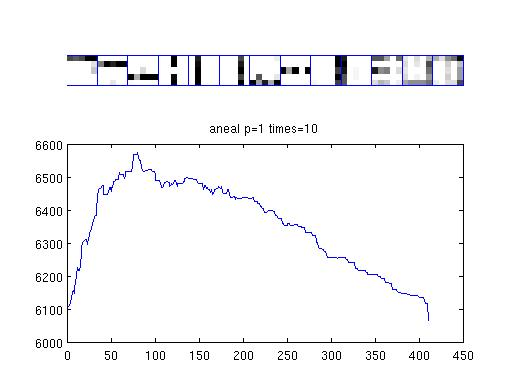
\includegraphics{anneal_10_1.jpg}} &
     \resizebox{40mm}{!}{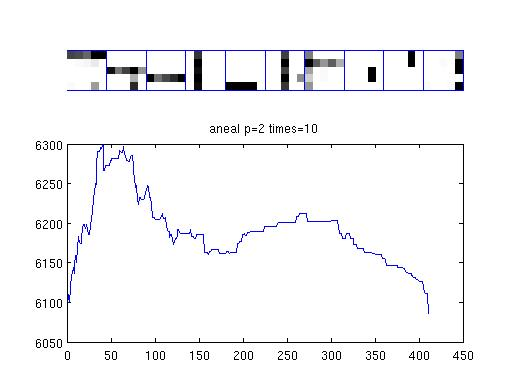
\includegraphics{anneal_10_2.jpg}}\\ 
     \resizebox{40mm}{!}{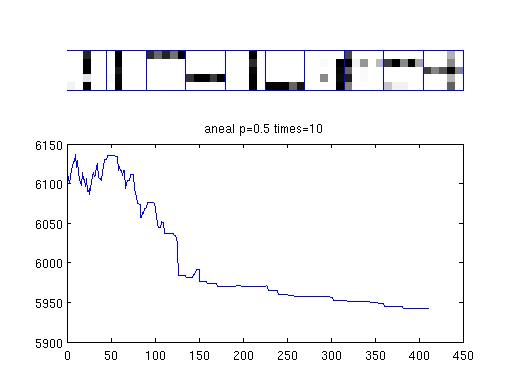
\includegraphics{anneal_10_05.jpg}} &
     \resizebox{40mm}{!}{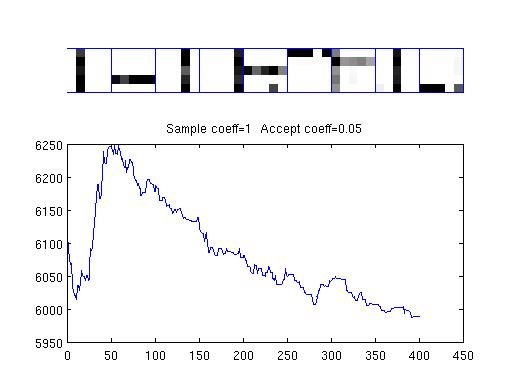
\includegraphics{hard.jpg}}\\
   \end{tabular}
    \caption{Down-Right is previous no-annealing result,the annealed ones(constant $r_{proposal}$) donot look good}
    \label{fig:by:table} 
\end{figure}
2) Annealed $r_{proposal}$;\\
Simply, I set $r_{proposal}$=$\frac{1}{T}$, where we want harder proposal assigment in the beginning and softer one later on.
\begin{figure}
 \centering
   \begin{tabular}{ccc}    
     \resizebox{40mm}{!}{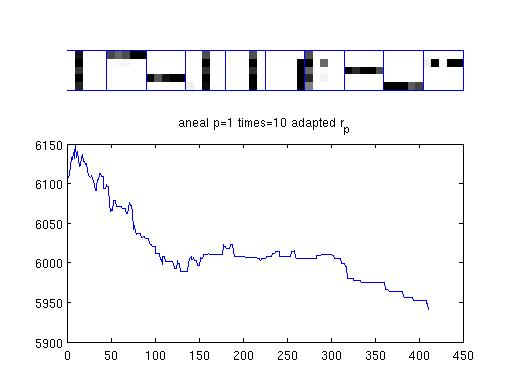
\includegraphics{anneal_10_1_a.jpg}} &
     \resizebox{40mm}{!}{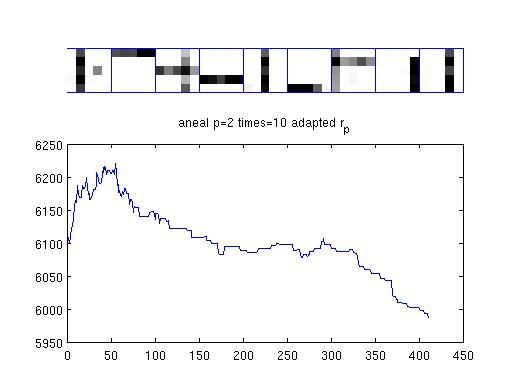
\includegraphics{anneal_10_2_a.jpg}}\\ 
     \resizebox{40mm}{!}{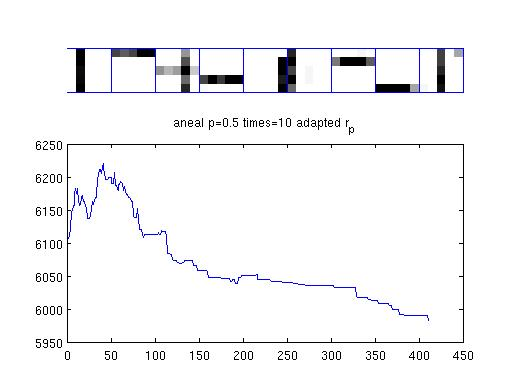
\includegraphics{anneal_10_05_a.jpg}} &
     \resizebox{40mm}{!}{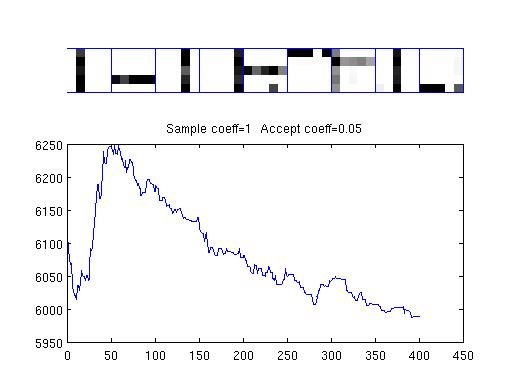
\includegraphics{hard.jpg}}\\
   \end{tabular}
    \caption{Using annealed $r_{proposal}$, p=1 is even better than the no-annealed one(down-right) by finding right number bars}
    \label{fig:by:table} 
\end{figure}
\newpage
\subsection{ii)Annealed Local-table and Merge Dish:}
From Figure 3, we can see that:\\ \\
1) annealing merge dish(right) can be also useful to prevent mixture of bars;\\
2) annealing local table(left) is harmful to prevent tables from communicating with each other;\\
\begin{figure}
 \centering
   \begin{tabular}{ccc}    
     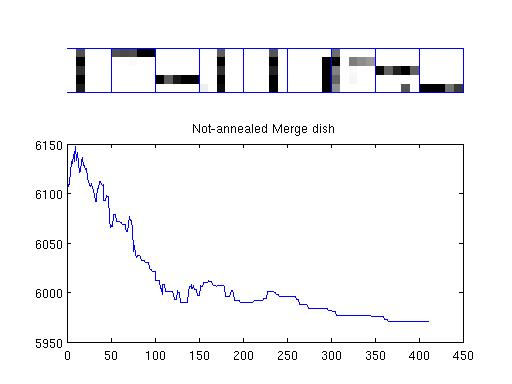
\includegraphics[width=2in,height=2in]{not_anneal_md.jpg} &
     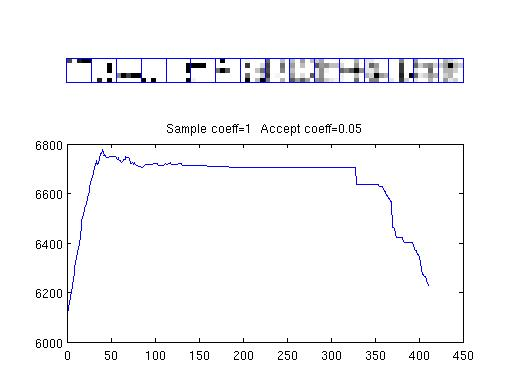
\includegraphics[width=2in,height=2in]{anneal_lt.jpg} &
     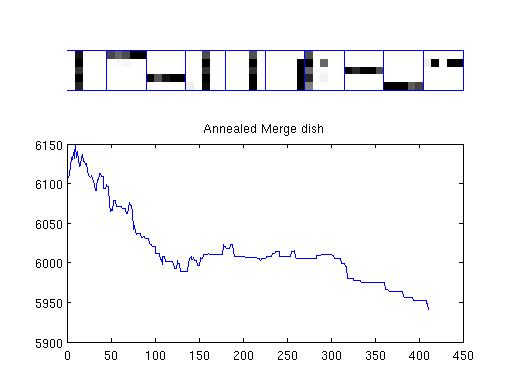
\includegraphics[width=2in,height=2in]{anneal_md.jpg} \\
   \end{tabular}
    \caption{(left)no anneal local-table,merge-dish;(mid)anneal local-table only(right)anneal merge-dish only}
    \label{fig:by:table} 
\end{figure}


\end{spacing}
\end{document}

%%%%%%%%%%%%%%%%%%%%%%%%%%%%%%%%%%%%%%%%%%%%%%%%%%%%%%%%%%%%%
